\documentclass[paper]{ieicej}
%\documentclass[invited]{ieicej}% 招待論文
%\documentclass[survey]{ieicej}% サーベイ論文
%\documentclass[comment]{ieicej}% 解説論文
%\usepackage[dvips]{graphicx}
%\usepackage[dvipdfmx]{graphicx,xcolor}
\usepackage[dvipdfmx]{graphicx}
\usepackage[fleqn]{amsmath}
\usepackage{newtxtext}% 英数字フォントの設定を変更しないでください
\usepackage[varg]{newtxmath}% % 英数字フォントの設定を変更しないでください
\usepackage{latexsym}
\usepackage{otf}%たつさき

\setcounter{page}{1}

\jtitle{テスト}
\jsubtitle{テスト2}
\etitle{test}
\esubtitle{test2}

\authorlist{%
\authorentry[imamura.yuuki475@mail.kyutech.jp]{今村 優希}{Yuki Imamura}{kyutech}
\authorentry[kawasaki.taiga711@mail.kyutech.jp]{川\UTF{FA11}  大雅}{Taiga Kawasaki}{kyutech}
% \authorentry[メールアドレス]{和文著者名}{英文著者名}{所属ラベル}
}
\affiliate[kyutech]{九州工業大学情報工学部 情報・通信工学科 3年\\ 福岡県飯塚市川津680-4}
  {Kyushu Institute of Technology\\ School of Computer Science and System Engineering\\ Department of Computer Science and Networks}
%\affiliate[所属ラベル]{和文勤務先\\ 連絡先住所}{英文勤務先\\ 英文連絡先住所}
\jalcdoi{???????????}% ← このままにしておいてください

\begin{document}
\begin{abstract}
%和文あらまし 500字以内
テスト
\end{abstract}
\begin{keyword}
%和文キーワード 4〜5語
VAE, FPGA, エッジコンピューティング
\end{keyword}
\begin{eabstract}
%英文アブストラクト 100 words
test
\end{eabstract}
\begin{ekeyword}
%英文キーワード
VAE, FPGA, edge computing
\end{ekeyword}
\maketitle

\section{はじめに}
近年,無線通信技術は飛躍的に向上しており,5G通信の普及が進んでいる.
5Gは従来の4Gなど通信規格と異なり,「高速大容量」「低遅延」「多数同時接続」の3つの特徴を備えており,その中でも「低遅延」と「多数同時接続」は新たな通信環境を構築する上で重要な軸となっている\cite{5g}.

従来の4G通信は,人が使用するスマートフォンや携帯に焦点を当てていた.
しかし,5Gでは車両,ドローン,センサなどのIoT機器が大量にネットワークに接続されることを前提としている.
このような環境においては,従来のクラウド中心の処理方式では,トラヒック増加による遅延や負荷集中が生じる可能性があり,5Gの利点を十分に発揮できない問題がある.
また,今現在のIT業界ではクラウドが主流で,処理の多くを一つ(もしくは複数の)コンピュータで行うという構造である.
多くの端末から取得したデータをクラウドのみで処理を行うのはある程度限界があり,またトラヒック量が増加して,5Gのメリットを享受できないという問題が発生すると考えられる.

このような課題を解決するため,エッジコンピューティングという技術が近年注目され始めている.
エッジコンピューティングとは,従来はクラウドで行っていた処理の一部を,ユーザ端末(スマートフォンやIoT機器)の近い位置である基地局やその至近に設置されているサーバなどでデータ処理を行う技術である\cite{edge-com}.
この技術を用いることでクラウドにかかる処理をエッジコンピューティングで分散することが可能で,通信のトラヒック量,5Gの特徴のひとつである「低遅延」に貢献することも可能である.

そこで,エッジコンピューティングの実現をVAEとFPGAを用いて実現することを考えた.
(本文を書きながら続きを記述予定)

\section{システム概要}
\subsection{全体}
本システムは,自動車の自動運転環境を想定し,エッジデバイスとしてFPGAを用いてVAEによる以下の2つの処理を行うものである.
\begin{enumerate}
\item 画像圧縮:FPGAに搭載されたVAEが入力画像を圧縮し,クラウドへ送信する.
\item 異常検知:FPGAが道路状況を解析し,異常を検知した場合に自動車側へ報告する.
\end{enumerate}
本報告では,実験を簡略化するためにグレースケール画像を使用し,MATLAB環境でシステムの一部をシミュレートした.また,VAEの活用はSDカード経由で「画像圧縮」「異常検知」「画像認識」の処理を実行する.

\subsection{VAE基本構造}
FPGAの物理的な制約を考慮して,入力ノード9個,中間層ノード2個,出力ノード9個で作成した.実行時は,512×512ピクセルの画像を処理するために9×2×9構造のVAEを繰り返し使用し,その結果を逐次加算していくことで最終的な出力を得る.入力層から中間層,中間層から出力までの処理をハードウェア(FPGA)が行い,中間層で生成された潜在変数の平均と分散の加算処理をソフトウェアで行う.

\begin{figure}[htbp]
    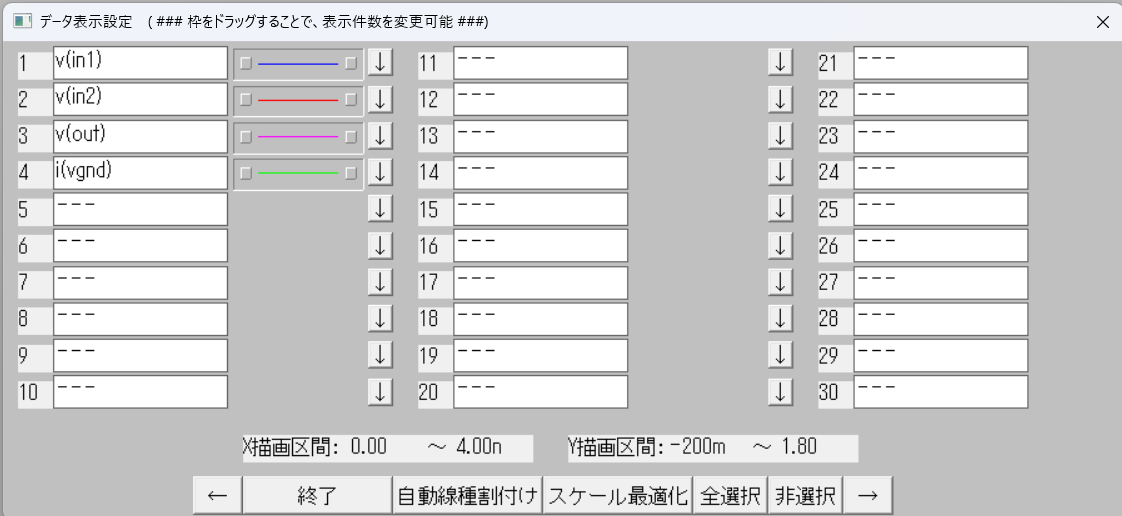
\includegraphics[width=0.9\columnwidth]{figures/test.png}
    \caption{テスト}
    \label{fig:test}
\end{figure}

\subsection{処理構造}



\section{実行環境}
開発言語はMATLAB,実行ハードウェアはFPGA(ZYNQ-7010)を用いる.入力データでは512×512のグレースケール画像を使用し,道路の様子を映した画像である.

\section{実行結果 及び 評価}

\section{考察}

\section{結論と今後の展望}
今回は,エッジコンピューティングを意識したVAEとFPGAの手法に関して報告を行った.

\ack
今回のシステム構築に対して,様々な支援を頂いた方々に感謝する.
これからも,日本や世界を支えるエンジニアになるために尽力する.
%\bibliographystyle{sieicej}
%\bibliography{myrefs}
\begin{thebibliography}{99}% 文献数が10未満の時 {9}
\bibitem{5g} 
森川博之, 5G次世代移動通信規格の可能性, 岩波書店, 
\bibitem{edge-com} 
田中裕也, 高橋紀之, 河村龍太郎, "IoT時代を拓くエッジコンピューティングの研究開発", NTT技法ジャーナル, vol.27, no.8, pp.59-63, 2015.
\end{thebibliography}

\end{document}
